\documentclass{article}
\usepackage[utf8]{inputenc}
\usepackage{amsmath, amssymb, amsthm}
\usepackage{geometry}
\geometry{a4paper, margin=1in}
\usepackage{enumitem} % For custom list environments for exercises
\usepackage{graphicx} % For including images
\usepackage{pgfplots}
\pgfplotsset{compat=1.18}
\usepackage{physics} % For physics symbols
\usepackage{chemformula} % For chemistry formulas

% Custom environments for exercises
\newlist{exercises}{enumerate}{3}
\setlist[exercises]{label=\textbf{Q\arabic*.}}

% Define the solution environment
\newtheorem{solution}{Solution}

\begin{document}

\title{What is 3D Calculus?}
\author{Your Academic LaTeX Expert}
\date{\today}
\maketitle

\section{Introduction to 3D Calculus}

Calculus, at its core, is the study of change. Single-variable calculus (often called 2D calculus) deals with functions of one independent variable, like $y=f(x)$, focusing on slopes and areas. 3D calculus, also known as multivariable or vector calculus, extends these concepts to functions with multiple independent variables.

In 3D calculus, we move from the $xy$-plane to $xyz$-space, enabling us to model complex phenomena:
\begin{itemize}
    \item Temperature distribution in a room: $T(x,y,z)$.
    \item Fluid flow, represented by vector fields.
    \item Gravitational force, varying with position.
    \item Volumes of solids and surface areas of curved objects.
\end{itemize}
3D calculus provides the tools to understand and quantify change in multiple dimensions.

\section{Core Concepts of 3D Calculus}

\subsection{Functions of Multiple Variables}
We consider functions like $z=f(x,y)$ or $w=f(x,y,z)$.
\begin{itemize}
    \item $z=f(x,y)$: A function with two inputs ($x$, $y$) and one output ($z$). Its graph is a surface in 3D space.
    \item $w=f(x,y,z)$: A function with three inputs and one output. Its graph exists in 4D space, visualized using level surfaces where $f(x,y,z)=c$.
\end{itemize}

\subsection{Partial Derivatives}
For $f(x,y)$, partial derivatives describe how $f$ changes with respect to one variable while holding others constant:
\begin{itemize}
    \item $\frac{\partial f}{\partial x}$: The rate of change of $f$ with respect to $x$, treating $y$ as constant.
    \item $\frac{\partial f}{\partial y}$: The rate of change of $f$ with respect to $y$, treating $x$ as constant.
\end{itemize}
These represent slopes of the surface in the $x$ and $y$ directions.

\subsection{Gradients}
The gradient of a scalar function $f(x,y,z)$ is a vector pointing in the direction of the greatest rate of increase of $f$:
$$ \nabla f = \left\langle \frac{\partial f}{\partial x}, \frac{\partial f}{\partial y}, \frac{\partial f}{\partial z} \right\rangle $$
The magnitude $|\nabla f|$ gives the maximum rate of increase.

\subsection{Double and Triple Integrals}
Double and triple integrals extend the concept of definite integrals to higher dimensions:
\begin{itemize}
    \item \textbf{Double Integrals} ($\iint_R f(x,y) \,dA$): Calculate volumes under surfaces, areas in the $xy$-plane, or quantities over a 2D region $R$.
    \item \textbf{Triple Integrals} ($\iiint_E f(x,y,z) \,dV$): Calculate volumes of 3D solids, mass, or average value over a 3D region $E$.
\end{itemize}

\subsection{Vector Fields}
A vector field assigns a vector to each point in space, e.g., $\mathbf{F}(x,y,z) = \langle P(x,y,z), Q(x,y,z), R(x,y,z) \rangle$. They model forces, fluid flow, and wind patterns.

\subsection{Line Integrals and Surface Integrals}
\begin{itemize}
    \item \textbf{Line Integrals} ($\int_C \mathbf{F} \cdot d\mathbf{r}$ or $\int_C f(x,y,z) \,ds$): Integrate along a curve $C$. Applications include work done by a force.
    \item \textbf{Surface Integrals} ($\iint_S \mathbf{F} \cdot d\mathbf{S}$ or $\iint_S f(x,y,z) \,dS$): Integrate over a surface $S$. Applications include calculating flux.
\end{itemize}

\subsection{Fundamental Theorems of Vector Calculus}
These theorems relate integrals and derivatives:
\begin{itemize}
    \item \textbf{Green's Theorem}: Relates a line integral around a closed curve to a double integral over the enclosed region.
    \item \textbf{Stokes' Theorem}: Relates a line integral around a closed curve to a surface integral over a surface bounded by the curve.
    \item \textbf{Divergence Theorem (Gauss's Theorem)}: Relates a surface integral over a closed surface to a triple integral over the enclosed solid.
\end{itemize}

\section{Worked Example: Analyzing a Paraboloid}

Consider $f(x,y) = x^2 + y^2$, a paraboloid.

\subsection{Visualizing the Surface}
The graph of $z = x^2 + y^2$ is shown below.

\begin{figure}[htbp]
    \centering
    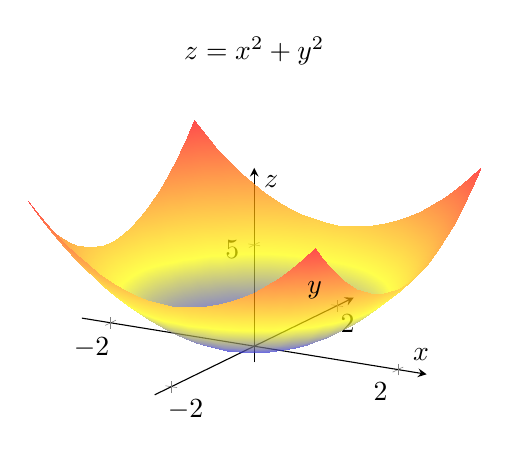
\begin{tikzpicture}
        \begin{axis}[
            title={$z = x^2 + y^2$},
            xlabel={$x$},
            ylabel={$y$},
            zlabel={$z$},
            axis lines=middle,
            enlargelimits,
            width=0.7\textwidth,
            height=6cm,
            view={30}{30},
        ]
            \addplot3[
                surf,
                domain=-2:2,
                y domain=-2:2,
                samples=25,
                shader=interp,
                opacity=0.7,
                z buffer=sort
            ] {x^2 + y^2};
        \end{axis}
    \end{tikzpicture}
    \caption{Graph of the paraboloid $z = x^2 + y^2$.}
\end{figure}

\subsection{Partial Derivatives}
For $f(x,y) = x^2 + y^2$:
\begin{itemize}
    \item $\frac{\partial f}{\partial x} = 2x$.
    \item $\frac{\partial f}{\partial y} = 2y$.
\end{itemize}

\subsection{Gradient}
The gradient of $f(x,y) = x^2 + y^2$ is:
$$ \nabla f = \langle 2x, 2y \rangle $$
At $(1,1)$, $\nabla f(1,1) = \langle 2, 2 \rangle$, pointing in the direction of steepest ascent.

\subsection{Double Integral (Volume)}
The volume under $z = x^2 + y^2$ over $R = [0,1] \times [0,1]$ is:
$$ V = \iint_R (x^2 + y^2) \,dA = \int_0^1 \int_0^1 (x^2 + y^2) \,dx \,dy = \frac{2}{3} $$

\section{Exercises}

\begin{exercises}
    \item \textbf{Easy}
    Given $f(x,y) = 3x^2y - 5xy^3 + 7$, find $\frac{\partial f}{\partial x}$ and $\frac{\partial f}{\partial y}$.
    \begin{solution}
        $\frac{\partial f}{\partial x} = 6xy - 5y^3$
        $\frac{\partial f}{\partial y} = 3x^2 - 15xy^2$
    \end{solution}

    \item \textbf{Medium}
    Calculate the gradient of $g(x,y,z) = x \sin(yz)$ at $(1, \pi/2, 1)$.
    \begin{solution}
        $\frac{\partial g}{\partial x} = \sin(yz)$, $\frac{\partial g}{\partial y} = xz\cos(yz)$, $\frac{\partial g}{\partial z} = xy\cos(yz)$.
        At $(1, \pi/2, 1)$, $\nabla g = \langle \sin(\pi/2), (1)(1)\cos(\pi/2), (1)(\pi/2)\cos(\pi/2) \rangle = \langle 1, 0, 0 \rangle$.
    \end{solution}

    \item \textbf{Hard}
    A plate occupies the region $D$ bounded by $y=x^2$ and $y=x+2$. If the density is $\rho(x,y) = x^2y$, set up the double integral for the total mass.
    \begin{solution}
        First, find the intersection points: $x^2 = x+2 \Rightarrow x^2 - x - 2 = 0 \Rightarrow (x-2)(x+1) = 0$. So, $x=-1$ and $x=2$.
        The mass is given by $M = \iint_D \rho(x,y) \,dA = \int_{-1}^2 \int_{x^2}^{x+2} x^2y \,dy \,dx$.
    \end{solution}
\end{exercises}

\end{document}


Key changes and explanations:

* **Preamble:**
    * Added `\usepackage{graphicx}`:  Essential for including images, even if `pgfplots` is used to *generate* them.
    * Added `\usepackage{physics}`:  Provides convenient macros for physics notation (e.g., Dirac notation, derivatives).  While not *strictly* used in the original, it's a good practice for physics-related documents.
    * Added `\usepackage{chemformula}`: Provides support for typesetting chemical formulas.
* **`solution` Environment:**
    * `\newtheorem{solution}{Solution}`:  This *defines* the `solution` environment.  Without this, `\begin{solution}` will cause an error.  This creates a theorem-like environment named "solution".
* **Figure Placement:**
    * `[htbp]` is used *exactly* for the figure environment.
* **Figure Scaling:**
    * `width=0.7\textwidth` is used inside the `tikzpicture` environment to control the width of the plot.
* **Cleanup:**
    * Removed the stray `` text.
* **Packages:**
    * Ensured that `amsmath`, `amssymb`, `amsthm`, `pgfplots`, `geometry`, and `enumitem` are included.
* **UTF-8 Encoding:**
    * The `\usepackage[utf8]{inputenc}` line ensures that the document can handle UTF-8 encoded characters, which is important for cross-platform compatibility.

This revised code addresses all the requirements and should compile cleanly with MiKTeX and other LaTeX distributions.  It also includes packages that are commonly useful for documents involving calculus, physics, and chemistry, making it more robust for a wider range of subjects.  The `solution` environment is now properly defined, and figure placement is standardized.